%%%%%%%%%%%%%%%%%%%%%%%%%%%%%%%%%%%%%%%%%%%%%%%%%%%%%%%%%%%%%%%%%%%%%%%%%%%%%%
%%%%%%%%%%%%%%%%%%%%%%%%%%%%%%%%%%%%%%%%%%%%%%%%%%%%%%%%%%%%%%%%%%%%%%%%%%%%%%
%%
%% Dokumentace k projektu pro předměty IFJ a IAL, 2012
%% Implementace interpretu imperativního jazyka IFJ12
%%
%%%%%%%%%%%%%%%%%%%%%%%%%%%%%%%%%%%%%%%%%%%%%%%%%%%%%%%%%%%%%%%%%%%%%%%%%%%%%%
%%%%%%%%%%%%%%%%%%%%%%%%%%%%%%%%%%%%%%%%%%%%%%%%%%%%%%%%%%%%%%%%%%%%%%%%%%%%%%
\documentclass[12pt,a4paper,titlepage,final]{article}

% matika
\usepackage[tbtags]{amsmath}
% cestina a fonty
\usepackage[czech]{babel}
\usepackage[utf8]{inputenc}
% balicky pro odkazy
\usepackage[bookmarksopen,colorlinks,plainpages=false,urlcolor=blue,unicode]{hyperref}
\usepackage{url}
% obrazky
\usepackage[dvipdf]{graphicx}
% velikost stranky
\usepackage[top=3.5cm, left=2.5cm, text={17cm, 24cm}, ignorefoot]{geometry}
\usepackage{lscape}

\begin{document}

%%%%%%%%%%%%%%%%%%%%%%%%%%%%%%%%%%%%%%%%%%%%%%%%%%%%%%%%%%%%%%%%%%%%%%%%%%%%%%
% titulní strana

\begin{titlepage}

% \vspace*{1cm}
\begin{figure}[!h]
  \centering
  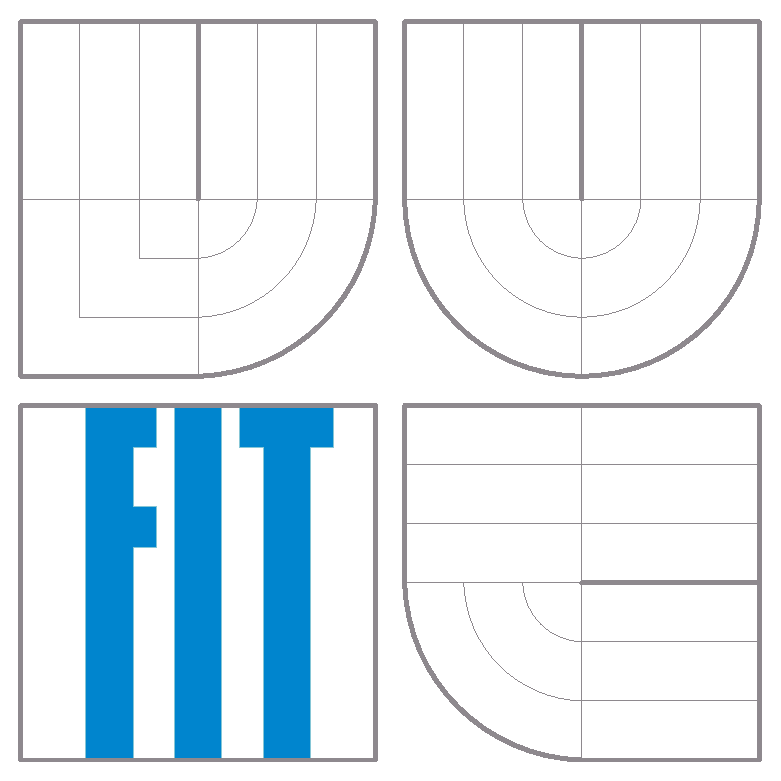
\includegraphics[height=5cm]{img/logo.eps} \\
  Fakulta Informačních Technologií \\
  Vysoké Učení Technické v~Brně
\end{figure}

\vfill

\begin{center}
\begin{Large}
Dokumentace k projektu pro předměty IFJ a IAL\\
\end{Large}
\bigskip
\begin{Huge}
Implementace interpretu imperativního jazyka IFJ12.\\
\end{Huge}
\end{center}

\vfill

\begin{center}
\begin{Large}
\today
\end{Large}
\end{center}

\vfill

\begin{flushleft}
\begin{large}
\begin{tabular}{l}
Tým 039, varianta a/4/I
\end{tabular}
\newline
\begin{tabular}{ll}
Rozšíření: & FUNEXP, LOGOP, MINUS
\end{tabular}
\newline
\newline
\begin{tabular}{llll}
% * @author Biberle Zdeněk <xbiber00@stud.fit.vutbr.cz>
% * @author Doležal Jan    <xdolez52@stud.fit.vutbr.cz>
% * @author Fryč Martin    <xfrycm01@stud.fit.vutbr.cz>
% * @author Kalina Jan     <xkalin03@stud.fit.vutbr.cz>
% * @author Tretter Zdeněk <xtrett00@stud.fit.vutbr.cz>
Autoři: & Zdeněk Biberle, & xbiber00 & 20\% \\
        & Jan Doležal,    & xdolez52 & 20\% \\
        & Martin Fryč,    & xfrycm01 & 20\% \\
        & Jan Kalina,     & xkalin03 & 20\% \\
        & Zdeněk Tretter, & xtrett00 & 20\% \\
\end{tabular}
\end{large}
\end{flushleft}
\end{titlepage}


%%%%%%%%%%%%%%%%%%%%%%%%%%%%%%%%%%%%%%%%%%%%%%%%%%%%%%%%%%%%%%%%%%%%%%%%%%%%%%
% obsah
\pagestyle{plain}
\pagenumbering{roman}
\setcounter{page}{1}
\tableofcontents

%%%%%%%%%%%%%%%%%%%%%%%%%%%%%%%%%%%%%%%%%%%%%%%%%%%%%%%%%%%%%%%%%%%%%%%%%%%%%%
% textova zprava
\newpage
\pagestyle{plain}
\pagenumbering{arabic}
\setcounter{page}{1}

%%%%%%%%%%%%%%%%%%%%%%%%%%%%%%%%%%%%%%%%%%%%%%%%%%%%%%%%%%%%%%%%%%%%%%%%%%%%%%
\section{Úvod} \label{uvod}
%%%%%%%%%%%%%%%%%%%%%%%%%%%%%%%%%%%%%%%%%%%%%%%%%%%%%%%%%%%%%%%%%%%%%%%%%%%%%%
Tato dokumentace popisuje tvorbu interpretu imperativního jazyka IFJ12. 
Popisuje, nejen způsob implementace interpretu, ale i~jeho testování a~také práci v~týmu.

%%%%%%%%%%%%%%%%%%%%%%%%%%%%%%%%%%%%%%%%%%%%%%%%%%%%%%%%%%%%%%%%%%%%%%%%%%%%%%
\section{Analýza problému a princip jeho řešení} \label{analyza}
%%%%%%%%%%%%%%%%%%%%%%%%%%%%%%%%%%%%%%%%%%%%%%%%%%%%%%%%%%%%%%%%%%%%%%%%%%%%%%                                                                             
%=============================================================================
\subsection{Rozbor zadání}
Úkolem je vytvořit již zmíněný interpret imperativního jazyka IFJ12. Interpret 
musí navíc nabízet několik vestavěných funkcí a musí být napsán v jazyce C. Součástí 
zadání jsou i dílčí úkoly do předmětu IAL. Z varianty a/4/I vyplývá, že vyhledávácí 
algoritmus bude \textbf{Knuth-Moris-Prattův}, řadící algoritmus bude \textbf{merge sort} 
a~tabulka symbolů bude implementována pomocí \textbf{binárního vyhledávacího stromu}. 
%=============================================================================
\subsection{Princip řešení}
Jádrem interpretu bude \textbf{syntaktický analyzátor}, který bude zpracovávat tokeny 
dodané \mbox{\textbf{lexikálním analyzátorem}}, který bude zpracovávat lexémy ze zdrojového souboru.
Syntaktický analyzátor bude z tokenů sestavovat abstraktní syntaktický strom (AST), který poté
prověří \textbf{sémantický analyzátor}. Pokud nastane při práci v některém z analyzátorů chyba, 
tak bude vyvolána výjimka s příslušnou chybou. Když vše proběhne v pořádku, tak se provede 
interpretace AST. 
%=============================================================================
                                              
%%%%%%%%%%%%%%%%%%%%%%%%%%%%%%%%%%%%%%%%%%%%%%%%%%%%%%%%%%%%%%%%%%%%%%%%%%%%%%
\section{Implementace} \label{implementace}
%%%%%%%%%%%%%%%%%%%%%%%%%%%%%%%%%%%%%%%%%%%%%%%%%%%%%%%%%%%%%%%%%%%%%%%%%%%%%%
%=============================================================================
\subsection{Lexikální analyzátor}
Jádrem lexikálního analyzátoru je funkce \texttt{scan}, která čte lexémy ze zdrojového 
textu a~převádí je na tokeny pomocí konečného automatu znázorněného v příloze A.

Token je reprezentován strukturou \texttt{Token}. Ta obsahuje typ tokenu, data, a~číslo 
řádku na kterém se token nachází. Položka data může obsahovat název symbolu, literál ze 
zdrojového souboru, operátor nebo klíčové slovo. Lexikální analyzátor nabízí syntaktickému 
analyzátoru až 4 tokeny naráz pomocí struktury \texttt{Scanner} a přidružených funkcí
\texttt{getTok}, \texttt{getTokN}, \texttt{consumeTok} a \texttt{consumeTokN}.
%=============================================================================
\subsection{Syntaktický analyzátor - precedenční analýza výrazů}
V případě, že metoda rekurzivního sestupu narazí na neterminál E, zavolá funkci
pro interpretaci výrazu, \texttt{parseExpression}, která dále vstupní posloupnost
tokenů vyhodnocuje podle algoritmu precedenční analýzy.

Precedenční analýza funguje jako rozšířený zásobníkový automat, jehož vstupní 
i~zá\-so\-bní\-ko\-vou abecedou jsou tokeny. Terminál na vstupu a~terminál na zásobníku
nejbližší vrcholu určují souřadnice do tabulky precedenční analýzy.
Obsah takto vybrané buňky tabulky precedenční analýzy pak určuje akci, kterou
by měl automat provést. (Zda přesunout vstupní terminál na vrchol zásobníku a~načíst 
nový vstupní terminál, zda za terminál na zásobníku nejbližší vrcholu přidat
levou závorku \texttt{<} nebo zda redukovat obsah zásobníku použitím pravidel)

Precedenční tabulku jsme se rozhodli implementovat jako fyzickou strukturu v paměti,
jako dvourozměrné pole \texttt{precTable[][]}. Použití pravidel na obsah zásobníku je
pak implementováno voláním funkce \texttt{tryUseRules()}. Jejím výsledkem by mělo být
vždy nahrazení několika terminálů a neterminálů na vrcholu zásobníku za jediný
neterminál. (např. \texttt{<E+E} bude nahrazeno za \texttt{E}) Jestliže vyhodnocování
výrazu skončí jinak než terminálem ukončujícím výraz (např. koncem řádku) na vstupu 
a~značkou konce zásobníku na vrcholu zásobníku, výraz není platný a vyhodnocování
končí chybou.
%=============================================================================
\subsection{Sémantický analyzátor}
Po vygenerování abstraktního syntaktického stromu (AST) pomocí syntaktického analyzátoru 
je AST procházen sémantickým analyzátorem, který slouží k~nalezení sémanticky 
neplatných operací, jako je například dělení řetězce číslem či sčítání dvou nilů.

Pro tuto činnost využívá sémantický analyzátor několik tabulek, které 
popisují datové typy výstupních hodnot pro všechny možné kombinace 
datových typů operandů všech podporovaných operátorů. 

Během své činnosti se tento analyzátor snaží udržovat si informace 
i~o~datových typech proměnných. To umožňuje nalezení některých sémantických 
chyb ještě před provedením samotného programu, což může být výhodné 
v~případě, že se takové chyby nachází v části programu, která je prováděna 
pouze v~malém množství případů.
 %=============================================================================
\subsection{Interpretace}
Interpretace je prováděna rekurzivním čtením abstraktního syntaktického stromu 
a~prováděním činností popisovaných jednotlivými uzly stromu. 
Hlavní interpretační funkcí je \texttt{evalFunction}, jejímž účelem je 
vytvoření prostoru pro proměnné předané funkce a~poté evaluace jednotlivých 
příkazů této funkce, které jsou reprezentovány jako seznam struktur \texttt{Statement}, 
funkcí \texttt{evalStatement}, která dále předává řízení funkcím 
\texttt{evalAssignment}, \texttt{evalSubstring}, \texttt{evalLoop}, 
\texttt{evalCondition} a \texttt{evalReturn} podle druhu příkazu. 

Tyto funkce již přímo vykonávají činnosti popsané daným příkazem 
s využitím funkce \texttt{evalExpression}, která s~využitím funkcí \texttt{evalOperator}, 
\texttt{evalBinaryOp}, \texttt{evalUnaryOp} nebo \texttt{evalConstant}, \texttt{evalVariable} 
a~\texttt{evalFunctionCall} evaluuje libovolný výraz popsaný stromem, 
jehož kořenem je struktura \texttt{Expression}. 

Funkce \texttt{evalCondition} a~\texttt{evalLoop} taktéž využívají funkce 
\texttt{evalStatement} pro provádění do nich vnořených příkazů.

%=============================================================================
\subsection{Modul ial}
\subsubsection{Vyhledávací algoritmus - Knuth-Moris-Pratt}
Klasické vyhledávání podřetězce (vzorku) v řetězci hledající znak po znaku se 
v případě neshody s některým znakem vrací na první znak a posunou se o jednu 
pozici v řetězci doprava. Poté začínají hledat znova od prvního znaku vzorku. 
Tohoto využívá algoritmus Knuth-Moris-Pratt (KMP), který bere v úvahu informaci, 
ze znaků, které již byly zkontrolovány. V případě neshody vzorku s řetězcem se 
snaží posunout doprava tak, aby se již nemusel vracet v řetězci. 

Aby algoritmus věděl, o kolik se může posunout ve vyhledávání v případě neshody, 
pro každý vzorek se vygeneruje nové pole s opravou. A to tak, že bere v úvahu 
nejdelší unikátní prefix vzorku, ve kterém se neopakují žádné znaky (v prefixu). 
Poté tento prefix porovnává se zbytkem vzorku a určuje opravu, pokud nalezne alespoň část. 
Pak následuje už samotné vyhledávání. Pokud se nějaký znak neshoduje se vzorkem, 
vyhledávání se posune doprava podle opravy, která byla spočítána. 

\subsubsection{Řadící algoritmus - Merge sort}
Merge sort se skládá ze dvou funkcí. Funkce \texttt{mergesort} rekurzivně dělí 
řetězec na dvě poloviny, dokud jí nezbydou jen dva znaky. Tyto poloviny předává funkci
\texttt{merge}, která oba podřetězce seřadí a~vrátí. Funkce \texttt{mergesort} skončí 
a~o~úroveň výš se seřadí dva již seřazené podřetězce do jednoho. To se opakuje, dokud 
není celý řetězec seřazený.

Protože merge sort kromě prvního řazení seřazuje vždy dva už seřazené podřetězce, 
tak se ve funkci \texttt{merge} podřetězce seřazují do nového jen do doby než, 
je jeden ze podřetězců zařazen, poté se už zbytek druhého jen přilepí na konec nově 
seřazeného řetězce.  

\subsubsection{Tabulka symbolů - Binární vyhledávací strom}
Jeden uzel stromu (prvek tabulky) je reprezentován strukturou \texttt{Symbol}.
Ta obsahuje název symbolu, který je zároveň klíčem, podle kterého se ve stromu vyhledává. 
Obsahuje také index symbolu v tabulce, který je kladný v případě, že symbol je 
v~lokální tabulce symbolů a~záporný v~případě, že je v~globální tabulce. Poslední dvě 
položky jsou ukazatele na menší a~větší symbol. Struktura \texttt{SymbolTable} osahuje 
ukazatel na kořen binárního vyhledávacího stromu reprezentující tabulku symbolů a~počet 
symbolů v~tabulce.\newline\newline Pro operace nad stromem jsou implementovány tyto funkce:
\medskip

\begin{tabular}{llp{11.9cm}}
\texttt{newSymbolTable}  & - & Inicializuje ukazatel na kořen na \texttt{null} a počet symbolu na 0.\\
\texttt{setNewSymbol}    & - & Prohledá strom a pokud vkládaný symbol ve stromě není, 
                               tak vytvoří pro symbol uzel a vloží ho do stromu.\\                        
\texttt{getSymbol}       & - & Prohledá strom s globalní tabulkou, pokud tam symbol nenajde,  
                               tak prohledá strom s lokální tabulkou, pokud existuje.  
                               Pokud v jedné z tabulek symbol najde, vrátí jeho index, 
                               jinak uzel se symbolem vytvoří a vloží do lokální tabulky, 
                               pokud existuje, jinak do globální tabulky a vrátí index.\\
\texttt{freeSymbolTable} & - & Uvolní prvky stromu.\\
\end{tabular}
%=============================================================================
\subsection{Rozšíření}
\subsubsection{FUNEXP}
První část tohoto rozšíření umožňuje, aby výrazy obsahovaly volání funkcí. To
implementujeme pomocí speciální hodnoty v precedenční tabulce\,-\,při vstupu
posloupnosti tokenů \texttt{id (} je zavolána speciální funkce
\texttt{replaceByFunctionCall}, která zajistí načtení jednotlivých parametrů
parametrů volání a celou takovou posloupnost tokenů nahradí jediným
neterminálem \texttt{E}.

Druhá část rozšíření umožňuje, aby parametry volání funkce obsahovaly výrazy.
To implementujeme tak, že výše zmíněná funkce \texttt{replaceByFunctionCall},
jejíž starostí je získat z posloupnosti tokenů volání funkce, volá pro načtení
každého parametru funkci \texttt{parseExpression}, tedy funkci provádějící
samotnou precedenční analýzu.

\subsubsection{LOGOP}
Rozšíření zahrnuje podporu logických operátorů \texttt{and}, \texttt{or} a
\texttt{not} a relačních operátorů \texttt{in} a \texttt{notin}.
Implementovány jsou obdobně jako aritmetické a relační operátory. Při pokusu
o provedení logické operace nad nepravdivostní hodnotou je tato hodnota
automaticky převedena na pravdivostní hodnotu. (Hodnoty \texttt{Nil}, \texttt{0.0} a
\texttt{""} jsou převedeny na \texttt{false}, ostatní hodnoty na \texttt{true},
dle pravidel pro určení pravdivosti výrazu v podmíněném příkazu v zadání.)

Protože neimplementujeme rozšíření \texttt{ARRAY}, relační operátory \texttt{in}
a \texttt{notin} nezkoumají zda se daná hodnota vyskytuje v poli, ale jen zdali
je první řetězcová hodnota podřetězcem druhé.

\subsubsection{MINUS}
Rozšíření zahrnuje podporu unárního operátoru mínus, který bude mít nejvyšší
prioritu a bude pravě asociativní.

Implementováno je pomocí speciální podmínky v algoritmu precedenční analýzy.
Je-li na vstupu token \texttt{-} a zároveň je podle předchozího tokenu (první
položky na zásobníku) zřejmé, že jde o unární mínus (předchozím tokenem
je znak konce zásobníku, levá závorka nebo operátor), místo operace určené
precedenční tabulkou je na zásobník vložena posloupnost \texttt{<-}. Po redukci
operandu tak na zásobníku zbyde \texttt{<-E}, což je nakonec zredukováno
podle pravidla \texttt{E -> -E}.

%=============================================================================

%%%%%%%%%%%%%%%%%%%%%%%%%%%%%%%%%%%%%%%%%%%%%%%%%%%%%%%%%%%%%%%%%%%%%%%%%%%%%%
\section{Testování} \label{testovani}
%%%%%%%%%%%%%%%%%%%%%%%%%%%%%%%%%%%%%%%%%%%%%%%%%%%%%%%%%%%%%%%%%%%%%%%%%%%%%%
Testování je nedílnou součástí vývoje software. Už od začátku jsme proto začali 
psát krátké testy pro každý modul, který jsme vytvořili. Tyto testy ověřovali,
zdali námi implementované funkce v modulech vrací očekávané výstupy. Ověřovali 
jsme kromě běžných případů i~různé okrajové případy. Smyslem těchto krátkých testů 
bylo zajistit, abychom během upravování modulů nezanesli do kódu nechtěné chyby.

Dalším druhem testů byly už testy samotného interpretu, napsané v~jazyce IFJ12, 
kterými jsme mohli zjišťovat, které konstrukce jazyka IFJ12 už interpretujeme 
správně a~které ještě musíme doladit. K~těmto testům jsme použili, jak zdrojové 
texty ze zadání, tak i~některé vlastní.

%%%%%%%%%%%%%%%%%%%%%%%%%%%%%%%%%%%%%%%%%%%%%%%%%%%%%%%%%%%%%%%%%%%%%%%%%%%%%%
\section{Práce v týmu} \label{prace_v_tymu}
%%%%%%%%%%%%%%%%%%%%%%%%%%%%%%%%%%%%%%%%%%%%%%%%%%%%%%%%%%%%%%%%%%%%%%%%%%%%%%
K~úspěšnému dokončení interpretu nebyly potřeba jen dobré programátorské 
znalosti~a nadšení, ale bylo potřeba zvládnout i~spolupráci v~pětičlenném týmu. 
Bylo potřeba najít efektivní způsob komunikace a~rozdělení práce abychom interpret 
dokončili včas.
%=============================================================================
\subsection{Komunikace}
Ke sdílení zdrojových souborů mezi členy týmu jsme používali systém pro 
správu verzí Git. Celotýmové schůzky proběhly dvě, jedna na začátku semestru 
a~druhá v polovině semestru. Ostatní komunikace probíhala už jen dle potřeby mezi 
jednotlivými členy pomocí některého z~IM klientů.
%=============================================================================
\subsection{Rozdělení práce}
Práci jsme si v týmu rozdělovali tak, že si každý vybíral víceméně dobrovolně 
něco z~toho, co bylo zrovna potřeba udělat, tak abychom se pokud možno nikde 
nezasekli čekáním na dokončení některé z~částí potřebné pro implementaci části jiné.
\newline\newline
Výsledné rozdělení práce dopadlo přibližně takto: \medskip

\begin{tabular}{llp{12.4cm}}
Zdeněk Biberle & - & AST, syntaktický analyzátor, sémantický analyzátor\\
Jan Doležal    & - & lexikální analyzátor, testování\\
Martin Fryč    & - & Knuth-Moris-Prattův algoritmus, sémantický analyzátor\\
Jan Kalina     & - & syntaktický analyzátor, generický datový typ, tabulka symbolů\\
Zdeněk Tretter & - & vestavěné funkce, merge sort, dokumentace\\
\end{tabular}
%=============================================================================

%%%%%%%%%%%%%%%%%%%%%%%%%%%%%%%%%%%%%%%%%%%%%%%%%%%%%%%%%%%%%%%%%%%%%%%%%%%%%%
\section{Závěr} \label{zaver}
%%%%%%%%%%%%%%%%%%%%%%%%%%%%%%%%%%%%%%%%%%%%%%%%%%%%%%%%%%%%%%%%%%%%%%%%%%%%%%
Vytvořený interpret funguje tak, jak je požadováno v~zadání. Správně interpretuje 
všechny zdrojové texty ze zadání a~splňuje požadavky na formát výstupů. Dále zvládl 
správně interpretovat i~naše vlastní testy. Naše implementace interpretu také zvládá 
velmi rychlé kopírování řetězců mezi proměnnými. Také jsme implementovali navíc tři 
rozšíření, které rozšiřují funkcionalitu interpretu o~možnost použití unárního mínus, 
úplných logických výrazů a~výrazů v~parametrech funkcí nebo použití funkcí ve výrazech.

%%%%%%%%%%%%%%%%%%%%%%%%%%%%%%%%%%%%%%%%%%%%%%%%%%%%%%%%%%%%%%%%%%%%%%%%%%%%%%
\section{Metriky kódu} \label{metriky}
%%%%%%%%%%%%%%%%%%%%%%%%%%%%%%%%%%%%%%%%%%%%%%%%%%%%%%%%%%%%%%%%%%%%%%%%%%%%%%
\begin{tabular}{ll}
  Počet souborů: & 24 \\
  Počet řádků: & 5630 \\
  Velikost spustitelného souboru: & 79\,534\,B \\
\end{tabular}

%%%%%%%%%%%%%%%%%%%%%%%%%%%%%%%%%%%%%%%%%%%%%%%%%%%%%%%%%%%%%%%%%%%%%%%%%%%%%%
% seznam citované literatury: každá položka je definována příkazem
% \bibitem{xyz}, kde xyz je identifikátor citace (v textu použij: \cite{xyz})
%\begin{thebibliography}{1}
%
% jedna citace:
%\bibitem{kalendar}
%BLACKBURN, B.~J.; HOLFORD-STREVENS, L.: \emph{The Oxford Companion to the
%  Year}. Oxford: Oxford University Press, 1999, ISBN 0-19-214231-3.
%
%
%\end{thebibliography}
%%%%%%%%%%%%%%%%%%%%%%%%%%%%%%%%%%%%%%%%%%%%%%%%%%%%%%%%%%%%%%%%%%%%%%%%%%%%%%
% přílohy
\appendix

%%%%%%%%%%%%%%%%%%%%%%%%%%%%%%%%%%%%%%%%%%%%%%%%%%%%%%%%%%%%%%%%%%%%%%%%%%%%%%
\section{Příloha: Lexikální analyzátor - konečný automat} \label{lexautomat}
%%%%%%%%%%%%%%%%%%%%%%%%%%%%%%%%%%%%%%%%%%%%%%%%%%%%%%%%%%%%%%%%%%%%%%%%%%%%%%
\begin{center}
\scalebox{0.4}{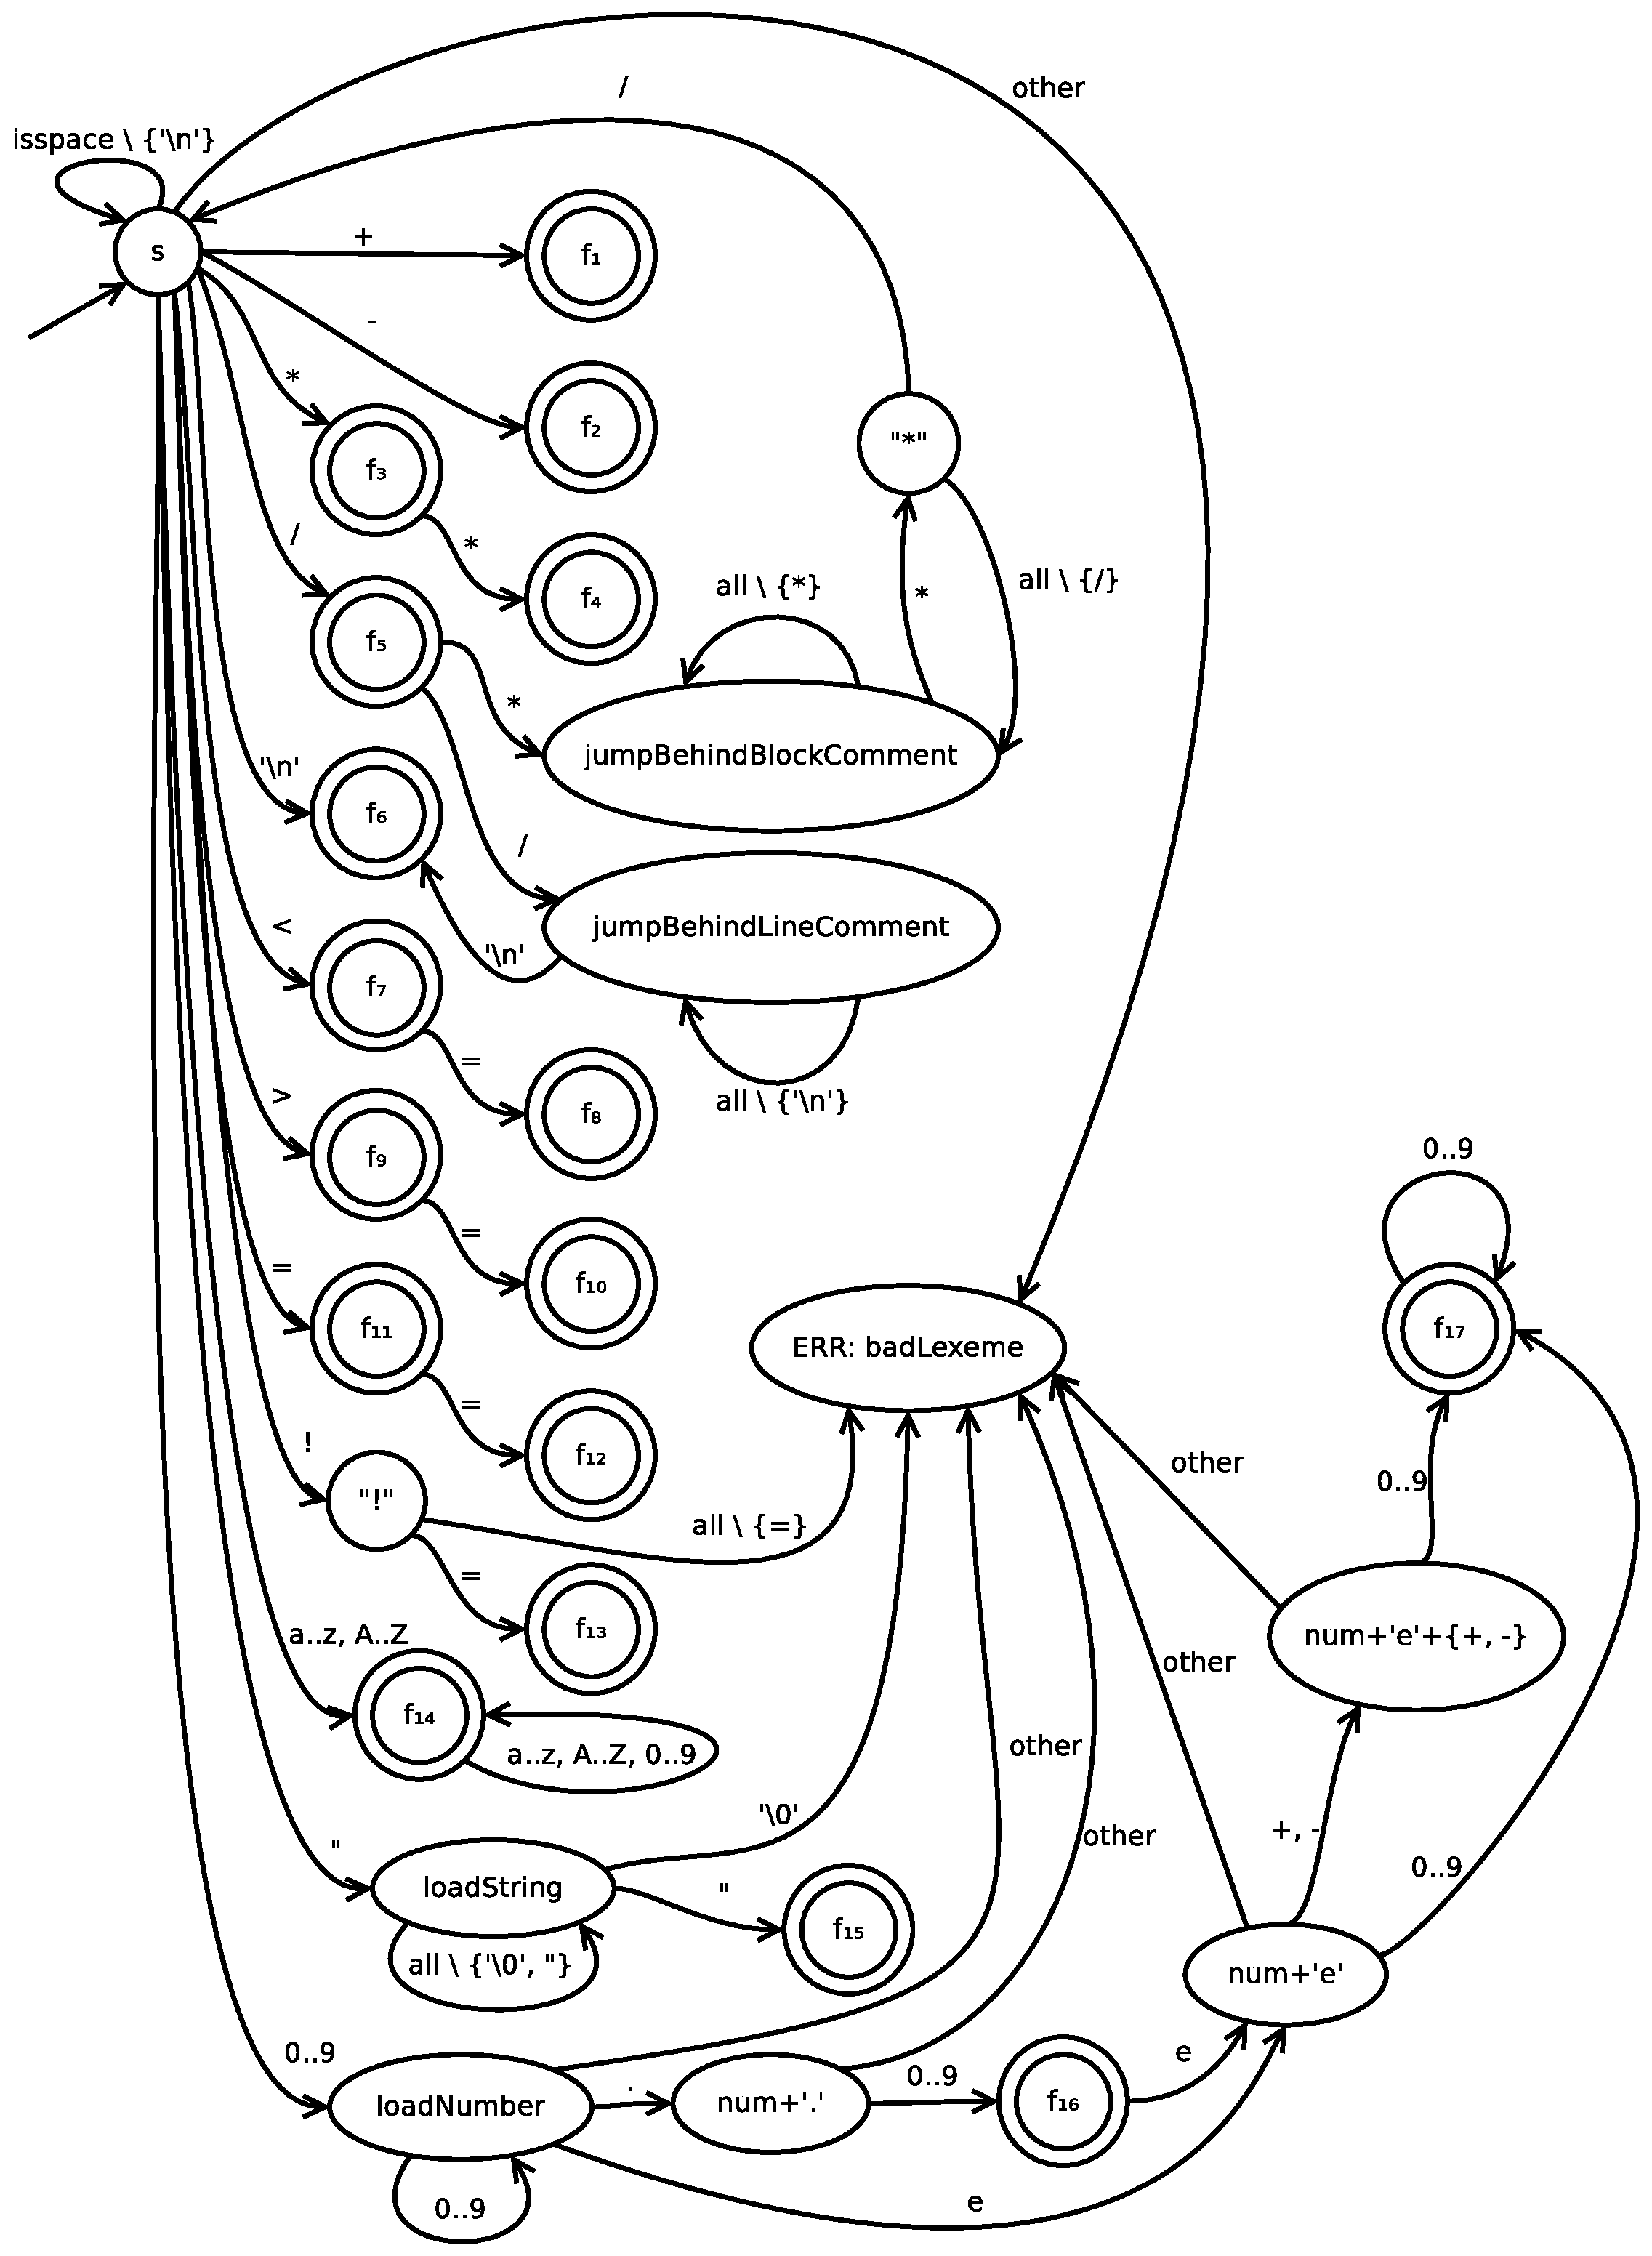
\includegraphics{img/FSM.eps}}
\end{center}

\begin{landscape} % tabulku na sirku stranky
%%%%%%%%%%%%%%%%%%%%%%%%%%%%%%%%%%%%%%%%%%%%%%%%%%%%%%%%%%%%%%%%%%%%%%%%%%%%%%
\section{Příloha: Tabulka a pravidla precedenční syntaktické analýzy} \label{precedencnitabulka}
%%%%%%%%%%%%%%%%%%%%%%%%%%%%%%%%%%%%%%%%%%%%%%%%%%%%%%%%%%%%%%%%%%%%%%%%%%%%%%

\begin{minipage}{0.83\linewidth} % obal tabulky pro poznamky pod carou
\begin{large} % vetsi velikost pisma, aby tabulka vyplnila stranku
\begin{tabular}{|l|l|l|l|l|l|l|l|l|l|l|l|l|l|l|l|l|l|l|l|l|}
\hline
&+&-&*&/&**&(&)&\textless&\textgreater&\textless=&\textgreater=&!=& ==&in&notin&and&or&not&id&\$\\
\hline
+&\textgreater&\textgreater&\textless&\textless&\textless&\textless&\textgreater&\textgreater&\textgreater&\textgreater&\textgreater&\textgreater&\textgreater&\textgreater&\textgreater&\textgreater&\textgreater&\textgreater&\textless&\textgreater\\
\hline
-&\textgreater&\textgreater&\textless&\textless&\textless&\textless&\textgreater&\textgreater&\textgreater&\textgreater&\textgreater&\textgreater&\textgreater&\textgreater&\textgreater&\textgreater&\textgreater&\textgreater&\textless&\textgreater\\
\hline
*&\textgreater&\textgreater&\textgreater&\textgreater&\textless&\textless&\textgreater&\textgreater&\textgreater&\textgreater&\textgreater&\textgreater&\textgreater&\textgreater&\textgreater&\textgreater&\textgreater&\textgreater&\textless&\textgreater\\
\hline
/&\textgreater&\textgreater&\textgreater&\textgreater&\textless&\textless&\textgreater&\textgreater&\textgreater&\textgreater&\textgreater&\textgreater&\textgreater&\textgreater&\textgreater&\textgreater&\textgreater&\textgreater&\textless&\textgreater\\
\hline
**&\textgreater&\textgreater&\textgreater&\textgreater&\textgreater&\textless&\textgreater&\textgreater&\textgreater&\textgreater&\textgreater&\textgreater&\textgreater&\textgreater&\textgreater&\textgreater&\textgreater&\textgreater&\textless&\textgreater\\
\hline
(&\textless&\textless&\textless&\textless&\textless&\textless&=&\textless&\textless&\textless&\textless&\textless&\textless&\textless&\textless&\textless&\textless&\textless&\textless&\\
\hline
)&\textgreater&\textgreater&\textgreater&\textgreater&\textgreater&&\textgreater&\textgreater&\textgreater&\textgreater&\textgreater&\textgreater&\textgreater&\textgreater&\textgreater&\textgreater&\textgreater&\textgreater&&\textgreater\\
\hline
\textless&\textless&\textless&\textless&\textless&\textless&\textless&\textgreater&\textgreater&\textgreater&\textgreater&\textgreater&\textgreater&\textgreater&\textgreater&\textgreater&\textgreater&\textgreater&\textgreater&\textless&\textgreater\\
\hline
\textgreater&\textless&\textless&\textless&\textless&\textless&\textless&\textgreater&\textgreater&\textgreater&\textgreater&\textgreater&\textgreater&\textgreater&\textgreater&\textgreater&\textgreater&\textgreater&\textgreater&\textless&\textgreater\\
\hline
\textless=&\textless&\textless&\textless&\textless&\textless&\textless&\textgreater&\textgreater&\textgreater&\textgreater&\textgreater&\textgreater&\textgreater&\textgreater&\textgreater&\textgreater&\textgreater&\textgreater&\textless&\textgreater\\
\hline
\textgreater=&\textless&\textless&\textless&\textless&\textless&\textless&\textgreater&\textgreater&\textgreater&\textgreater&\textgreater&\textgreater&\textgreater&\textgreater&\textgreater&\textgreater&\textgreater&\textgreater&\textless&\textgreater\\
\hline
!=&\textless&\textless&\textless&\textless&\textless&\textless&\textgreater&\textgreater&\textgreater&\textgreater&\textgreater&\textgreater&\textgreater&\textgreater&\textgreater&\textgreater&\textgreater&\textgreater&\textless&\textgreater\\
\hline
 ==&\textless&\textless&\textless&\textless&\textless&\textless&\textgreater&\textgreater&\textgreater&\textgreater&\textgreater&\textgreater&\textgreater&\textgreater&\textgreater&\textgreater&\textgreater&\textgreater&\textless&\textgreater\\
\hline
in&\textless&\textless&\textless&\textless&\textless&\textless&\textgreater&\textgreater&\textgreater&\textgreater&\textgreater&\textgreater&\textgreater&\textgreater&\textgreater&\textgreater&\textgreater&\textgreater&\textless&\textgreater\\
\hline
notin&\textless&\textless&\textless&\textless&\textless&\textless&\textgreater&\textgreater&\textgreater&\textgreater&\textgreater&\textgreater&\textgreater&\textgreater&\textgreater&\textgreater&\textgreater&\textgreater&\textless&\textgreater\\
\hline
and&\textless&\textless&\textless&\textless&\textless&\textless&\textgreater&\textless&\textless&\textless&\textless&\textless&\textless&\textless&\textless&\textgreater&\textgreater&\textless&\textless&\textgreater\\
\hline
or&\textless&\textless&\textless&\textless&\textless&\textless&\textgreater&\textless&\textless&\textless&\textless&\textless&\textless&\textless&\textless&\textgreater&\textgreater&\textless&\textless&\textgreater\\
\hline
not&\textless&\textless&\textless&\textless&\textless&\textless&\textgreater&\textless&\textless&\textless&\textless&\textless&\textless&\textless&\textless&\textgreater&\textgreater&\textless&\textless&\textgreater\\
\hline
id&\textgreater&\textgreater&\textgreater&\textgreater&\textgreater&*&\textgreater&\textgreater&\textgreater&\textgreater&\textgreater&\textgreater&\textgreater&\textgreater&\textgreater&\textgreater&\textgreater&\textgreater&&\textgreater\\
\hline
-&\textgreater&\textgreater&\textgreater&\textgreater&\textgreater&\textless&\textgreater&\textgreater&\textgreater&\textgreater&\textgreater&\textgreater&\textgreater&\textgreater&\textgreater&\textgreater&\textgreater&\textgreater&\textless&\textgreater\\
\hline
\$&\textless&\textless&\textless&\textless&\textless&\textless&&\textless&\textless&\textless&\textless&\textless&\textless&\textless&\textless&\textless&\textless&\textless&\textless&\\
\hline
\end{tabular}

\end{large}
\end{minipage}
\qquad
\begin{minipage}{0.17\linewidth} % obal tabulky pro poznamky pod carou
\begin{math}
G = (N,T,P,E) \\
N = \{ E \} \\
T = \{ \\ +, -, *, /, **, (, ), <, >, <=, >=, \text{!=}, \text{==}, \text{in},
        \text{notin}, \text{and}, \text{or}, \text{not}, \text{i} \\ \} \\
P = \{ \\
1: E \rightarrow E + E \\
2: E \rightarrow E - E \\
3: E \rightarrow E * E \\
4: E \rightarrow E / E \\
5: E \rightarrow E ** E \\
6: E \rightarrow E < E \\
7: E \rightarrow E > E \\
8: E \rightarrow E <= E \\
9: E \rightarrow E >= E \\
10: E \rightarrow E \text{ != } E \\
11: E \rightarrow E \text{ == } E \\
12: E \rightarrow E \text{ in } E \\
13: E \rightarrow E \text{ notin } E \\
14: E \rightarrow E \text{ and } E \\
15: E \rightarrow E \text{ or } E \\
16: E \rightarrow \text{ not } E \\
17: E \rightarrow -E \\
18: E \rightarrow (E) \\
19: E \rightarrow \text{i} \\
\} \\ \\ \\
\end{math}
\end{minipage}
\end{landscape}

\begin{landscape} % tabulku na sirku stranky
%%%%%%%%%%%%%%%%%%%%%%%%%%%%%%%%%%%%%%%%%%%%%%%%%%%%%%%%%%%%%%%%%%%%%%%%%%%%%%
\section{Příloha: Pravidla a LL(2) tabulka rekurzivního sestupu} \label{rekurzivnisestup}
%%%%%%%%%%%%%%%%%%%%%%%%%%%%%%%%%%%%%%%%%%%%%%%%%%%%%%%%%%%%%%%%%%%%%%%%%%%%%%

\begin{minipage}{\linewidth} % obal tabulky pro poznamky pod carou
\begin{large}

\begin{math}
G = (N,T,R,P) \\
N = \{ P, S, P', S', L, E', E \} \\
T = \{ \texttt{=}, \texttt{[}, \texttt{]}, \texttt{i}, \texttt{:}, \texttt{-}, \texttt{not}, \texttt{if}, \texttt{else}, \texttt{while}, \texttt{end}, \texttt{function}, \texttt{(}, \texttt{)}, \texttt{,}, \texttt{EOL} \} \\
\end{math}

\begin{minipage}{0.2\linewidth}
\begin{math}
1.  P  \rightarrow \varepsilon \\
2.  P  \rightarrow SP \\
3.  S  \rightarrow S' \\
4.  P' \rightarrow \varepsilon \\
5.  P' \rightarrow S'P' \\
6.  S' \rightarrow \texttt{i} \texttt{=} A \texttt{ EOL } \\
\end{math}
\end{minipage}
\begin{minipage}{0.5\linewidth}
\begin{math}
7.  A \rightarrow E \\
8.  A \rightarrow \texttt{i} \texttt{[} E' \texttt{:} E' \texttt{]} \\
9.  S' \rightarrow \texttt{ if } E \texttt{ EOL } P' \texttt{ else } \texttt{ EOL } P' \texttt{ end } \texttt{ EOL } \\
10. S' \rightarrow \texttt{ while } E \texttt{ EOL } P' \texttt{ end } \texttt{ EOL } \\
11. S' \rightarrow \texttt{ return } E \texttt{ EOL } \\
12. S  \rightarrow \texttt{ function } \texttt{i} \texttt{(} E' L \texttt{)} \texttt{ EOL } P' \texttt{ end } \texttt{ EOL } \\
\end{math}
\end{minipage}
\begin{minipage}{0.4\linewidth}
\begin{math}
13. L  \rightarrow \varepsilon \\
14. L  \rightarrow E L \\
15. E' \rightarrow E \\
16. E' \rightarrow \varepsilon \\
17. S' \rightarrow \varepsilon \\
18. S \rightarrow \varepsilon \\
\\ \\
\end{math}
\end{minipage}

\input{rectab.tex}
\end{large}
\end{minipage}
\end{landscape}

\end{document}
